\documentclass{SPhdThesis}
\usepackage[mathscr]{euscript}
\usepackage{wrapfig}
\usepackage[]{hyperref}
\usepackage[]{verbatim}

% PDF and title properties.
\SgSetTitle{Reinforcement Learning for Function Discovery as a Workflow Construction Method}
\SgSetAuthor{Laura D'Arcy}
\SgSetAuthorDegrees{MSc Computing}
\SgSetYear{2018}
\SgSetDegree{MSc Computing}
\SgSetDepartment{Department of Computer Science}
\SgSetUniversity{Cardiff University}
\SgSetDeclarationDate{September 2018}

% The document.
\begin{document}
	\begin{frontmatter}
		\SgAddTitle%
		\SgAddDeclaration%
		\begin{acknowledgments}
Write your acknowledgments here.
\end{acknowledgments}%
		\begin{abstract}
write your abstract here.
\begin{comment}
Surface integration is an important step for automatic 3D reconstruction of real objects. The goal of a surface integration algorithm is to reconstruct a surface from a set of range images registered in a common coordinate system. Based on the surface representation used, existing algorithms can be divided into two categories: volume-based and mesh-based. Volume-based methods have been shown to be robust to scanner noise and small features (regions of high curvature) and can build water tight models of high quality. It is, however, difficult to choose the appropriate voxel size when the input range images have both small features and large registration errors compared to the sampling density of range images. Mesh-based methods are more efficient and need less memory compared to volume-based methods but these methods fail in the presence of small features and are not robust to scanning noise. \\

This paper presents a robust algorithm for mesh-based surface integration of a set of range images. The algorithm is incremental and operates on a range image and the model reconstructed so far. Our algorithm first, transform the model in the coordinate system of the range image. Then, it finds the regions of model overlapping with the range image. This is done by shooting rays from the scanner, through the vertices in the range image and intersecting them with the model. Finally, the algorithm integrates the overlapping regions by using weighted average of points in the model and the  range image. The weights are computed using the scanner uncertainty and helps in reducing the effects of scanning noise. To handle small features robustly the integration of overlapping regions is done by computing the position of vertices in the range image along the scanner's line of sight. Since for every point in a range image there is exactly one depth value, the reconstructed surface in the regions of high curvature will not have self-intersections.

\end{comment}
\end{abstract}%
		\SgAddToc%  Table of contents.
		\SgAddLof%  List of figures.
		%\SgAddLot%  List of tables.
		%\SgAddLoa%  List of algorithms.
	\end{frontmatter}
   
	\chapter{Introduction}

Distributed systems can be defined as: `a collection of autonomous computing elements that can appear to its users as a single coherent system' \cite{vanSteen2016}. Distributed systems are used in a wide variety of applications, including P2P networks, cluster computing, large financial systems, and CCTV networks. As these systems are composed of a large number of individual components, the order of accessing these separate services, or the workflow, is very important to the efficacy and efficiency of achieving the desired task. Tracking a specific car through a large CCTV network, for example, would be extremely time consuming to do manually. Automated workflow construction is therefore an important open question in the area of distributed systems. 

One potential solution to the automated workflow question is the use of reinforcement learning. Reinforcement learning is a relatively new field within the larger scope of machine learning. Along with RL, machine learning has two other major subtypes: supervised learning and unsupervised learning. Supervised learning methods, which include classification and linear regression, are given training data of inputs and outputs which are provided by a `knowledgeable external supervisor'. While supervised learning is a popular method that can produce very accurate results, it isn't easily scalable, as correctly labelled data becomes more difficult to source with more complex information. Unsupervised learning, on the other hand, finds structure within collections of unlabelled data. While unsupervised learning methods, such as deep learning and clustering, can work in real time and work with unlabelled data, the results aren't always as accurate as required.

Reinforcement learning (RL) is the third subset of machine learning. In reinforcement learning, a learning agent develops policies that map states of the environment to actions, in order to maximise a numerical reward. Unlike supervised learning, the agent is not given any labelled examples, and unlike unsupervised learning, reinforcement learning is given a reward when a desirable outcome is achieved. RL algorithms produce policies by interacting with the environment in a trial and error fashion, in real time. 

Reinforcement learning does not require any pre-provided training data, and does not need to discover any hidden structure. Reinforcement learning, simply put, decides the optimal actions given a situation to maximize reward. Reinforcement learning has been used for a variety of problems and situations, including playing the board game Go\cite{Silver2017}, cooling data centres \cite{DBLP:journals/corr/abs-1709-05077}, and finding the optimal medication dosing for new medicines\cite{7591355}. It can operate with only a minimal understanding of its environment's structure, does not need any previous examples of how to act, and can can adapt to environments that change behaviour over time. Most importantly, because reinforcement learning works with situations that involve delayed rewards, these algorithms will work optimally with distributed systems, where multiple services will need to be accessed to reach the desired goal.

The next chapter of this dissertation discusses the major aims and objectives for this project, and the third chapter gives an overview of the basic reinforcement learning knowledge that is necessary for the rest of the dissertation. The problem description section gives structure to the environment this project aims to solve, and the approach and application sections describe how the solution was found. Finally, the results, analysis, conclusion and reflection sections follow.







    \chapter{Aims and Objectives}
\begin{comment}

use RL to learn the most efficient workflow of a distributed system composed of separate services, whose actions are unknown. By using RL, no training set is required, and the correct workflow can be found through use.

To model a distributed system an environment will be made that uses basic mathematical operators as components, there will be a 'correct workflow' e.g initial value $+3.5/2$, and the algorithms will test warious combinations of these services to get the desired results. 

The objectives are to build these environments of different levels of detail, and implementing different algorithms to find these functions.
\end{comment}
The aim of this project is to use reinforcement learning to find the most efficient workflow of a distributed system. The distributed system is composed of separate services whose semantics are unknown. By using reinforcement learning, no training set is required, and the current workflow can be found through use. The simplest analogy to a distributed system is an environment where basic mathematical operators are the individual service components, and the `ideal workflow' is an arbitrary function that is hidden from the learning agent. Creating and solving this type of environment is the primary goal for this project.

The first objective is to design and build a basic environment. The environment should have a small number of discrete states and actions. It should give a reward at each timestep depending on whether or not the `goal' is achieved. This basic environment is discussed further in the problem description section.

The next objective is to implement a learning algorithm to find the workflow. The ideal algorithm depends on a number of characteristics of the environment itself, including whether states are discrete or continuous, whether or not the environment is episodic, and so on. The choice of algorithm also depends on the need for either an off-policy or on-policy solution, the need to balance accuracy over speed of solution, and so on. These details are explored in depth in the background materials section.

The final objective is to add further complexity to the problem. This can be added in multiple different ways. The most obvious would be to increase the number of actions in the environment. Additional algorithms could be implemented, or noise could be added to each environment to slow the learning process. All of these depend on the time available at the end of the project.



    \chapter{Background Material}
\begin{comment}

\item RL Sutton book
\item deepmind lectures

\end{comment}

In order to correctly design the environments and implement reinforcement learning algorithms effectively, a certain amount of terminology needs to be understood. The first section of this chapter gives an overview of the basic terminology used within the reinforcement learning field. The second section discusses Markov decision processes, the mathematical framework used to formalize all reinforcement learning problems. In the final section of this chapter, the algorithms used in the rest of the dissertation are introduced. It is important to note this is only a brief overview of some basic concepts within reinforcement learning, for more detail please refer to Sutton and Barto's `Reinforcement Learning: An Introduction' \cite{Sutton:RLIntro01}.

\section{Basic Terminology}
Reinforcement learning is defined by the following:
\begin{quote}
A \textit{learning agent} interacts with its \textit{environment} by choosing \textit{actions} that affect the \textit{state} of the environment, and the eventual \textit{reward}. The agent seeks to develop a \textit{policy} that maximises reward by mapping states to the optimal actions.
\end{quote}
This definition has a few basic terms that need to be accurately described.

The \textit{learning agent} is the problem solver or operator itself, and the \textit{environment} is what this agent interacts with. In a game of chess, the player would be the agent, and the chess board would be the environment. An agent can have complete or incomplete control over its environment. For example, in chess the player can move its own pieces wherever it likes (within the constraints of the game - a bishop can only move diagonally and the king can only move one square at a time), but it cannot move the opponent's pieces, giving the agent incomplete control over the environment.

The \textit{actions} are simply that, the actions the agent can make at a given timestep. These actions affect the \textit{state} of the environment (positioning of pieces on a chess board). In this dissertation, as in many RL problems, we work with a special case where at every state the same set of actions can be performed - the action space is the same throughout the state space. 

Actions affect the state of the environment as well as the reward, both immediate and eventual. The \textit{reward} is a scalar value given at each timestep. In a game of chess, this could be 0 for each non-terminal move, 1 if the game results in a win, -1 if a loss and 0 for a stalemate. For a solution that requires reaching a goal state in the smallest amount of timesteps (such as golf), each timestep could provide a reward of -1 until the goal state is reached. A faster solution would then have a higher cumulative reward. Problems that don't have a terminal state are called continuous cases, and require slightly different treatment than cases with terminal states. In these cases a balance between valuing long term and short term reward must be found, and often require different mathematical treatment than cases with terminating states. Environments that terminate after a finite number of timesteps are called episodic cases, and are the type of cases that will be examined throughout this dissertation. 

A \textit{policy} is a function (either deterministic or stochastic) that maps states to actions in order to maximise cumulative reward. In tabular cases (those which have a finite set of discrete states and a finite set of discrete actions), the policy can often be represented as a matrix or dictionary, where each action within each state is given a probability for its selection. Often this policy is deterministic - the probabilities of all actions are 0 for a given state except for the action (or actions) that will bring the most reward, which would have a probability of 1 (or are given equal weights that sum to 1) - this is called a $greedy$ policy. Other policies are stochastic - even the actions considered less valuable have a non-zero chance of being chosen. These policies are often used because a learning algorithm needs to explore multiple paths to see if there is a possible reward resulting from an action. This is often termed `exploration vs exploitation' - policies often need to balance exploration - determining which algorithms are best, with exploitation - receiving the best possible reward. The most common type of stochastic policy is the $\varepsilon$-greedy function. $\varepsilon$-greedy functions act as greedy functions for the majority $1-\varepsilon$ of action choices, but for the remaining $\varepsilon$ all actions are chosen from with equal probability. Different policy types are used in different learning algorithms, as will be shown in section \ref{algorithms}.

\section{Markov Decision Processes}\label{MDP}
Markov decision processes (MDPs) are "a mathematically idealized form of the reinforcement learning problem for which precisely theoretical statements can be made".

By defining a problem using this framework, algorithms can be applied that are used throughout the reinforcement learning field. He we will re-frame some terms explained in the previous section under the MDP framework and provide their mathematical notation, as well as introduce some more concepts, before applying them to algorithms in the next section.

\begin{figure}[h]
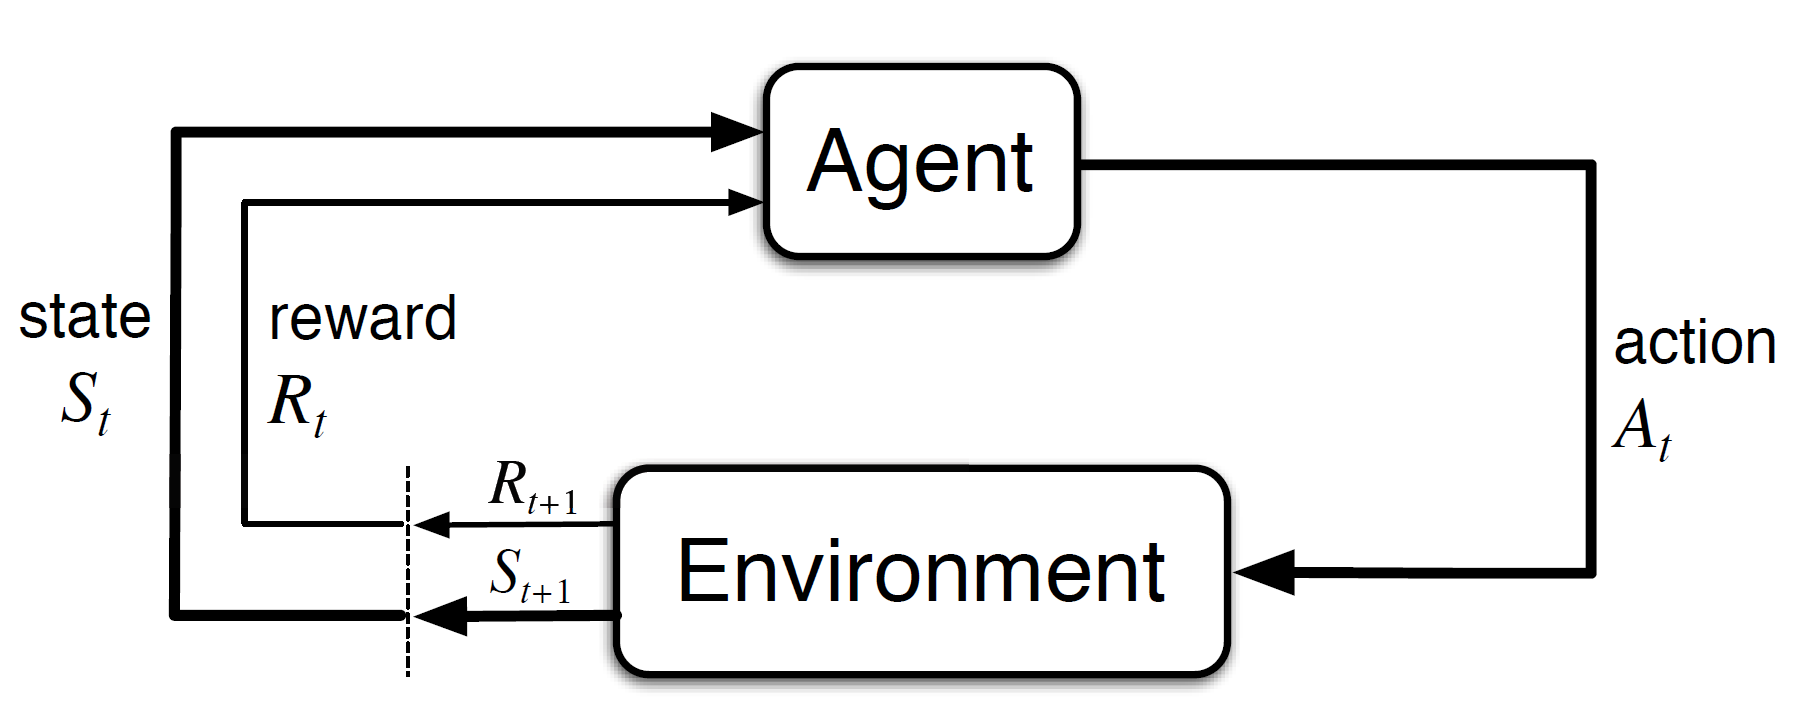
\includegraphics[width=\textwidth]{images/mdp}
\caption[Markov Decision Process]{graph displaying MDP taken from Sutton book}
\label{fig:mdp}
\end{figure}

MDPs frame an RL problem as seen in figure \ref{fig:mdp}. At each time step $t = 0\mathrm{,}1\mathrm{,}2\mathrm{,}3\mathrm{...}$ the agent receives information about the environment's state $S_{t}\in\mathscr{S}$, and selects an action $A_{t}\in\mathscr{A}$ based on the policy $\pi\left(A_t\mid S_t\right)$. At the next timestep, the agent receives a reward $R_{t+1}\in\mathscr{R}\subset\mathbb{R}$ and is in a new state $S_{t+1}$. This trajectory then continues: $S_0,A_0,R_1,S_1,A_1,R_2,S_2,A_2...$ until the episode terminates. 

The dynamics of a finite MDP (which has a finite set of states, actions, and rewards) is defined as a probability:
\begin{gather}
p(s',r\mid s,a) \doteq Pr\left\lbrace S_t=s',R_t=r \mid S_{t-1} = s, A_{t-1}=a\right\rbrace \\
\textnormal{where } p:\mathscr{S}\times\mathscr{R}\times\mathscr{S}\times\mathscr{A}\to\left[0,1\right] \nonumber \\
\textnormal{and } \sum_{s'\in\mathscr{S}}\sum_{r\in\mathscr{R}}p(s',r\mid s,a)=1, \textnormal{ for all }  s\in\mathscr{S},a\in\mathscr{A}\left(s\right) \nonumber
\end{gather}

These probabilities should completely characterise the dynamics of the environment in an ideal MDP. This means that states within the environment should have the \textit{Markov property}, which means the state must include all of the information needed to determine the next state and reward given the action selected - the history of all previous states can be thrown away and all important information must remain in the current state. An example of this is a toy helicopter. The state must include the current position and velocity of the helicopter in order to correctly determine the position of the helicopter in the next state. If the state included only position, it would either have to look to the previous state to calculate velocity, and therefore not be Markov (it cannot use history), or will not have enough information to determine the position of the next timestep. While useful from a theoretical standpoint to prove convergence of learning algorithms, in application of reinforcement learning, the Markov property can make solutions too computationally expensive, as will be discussed later on.

For episodic cases, the return $G_t$ is the sum of all rewards that have been given during the episode:
\begin{equation}
G_t \doteq R_{t+1}+R_{t+2}+R_{t+3}+...+R_T
\end{equation}

In many cases, immediate reward is considered more valuable than potential reward later on, so we can introduce a discount factor $\gamma\in\left(0,1\right]$:
\begin{equation}
G_t \doteq R_{t+1}+\gamma R_{t+2}+\gamma^2R_{t+3}+...+R_T = \sum^{\infty}_{k=0}\gamma^kR_{t+k+1}
\end{equation}
\begin{equation}
G_t = R_{t+1} + \gamma G_{t+1}
\end{equation}

A unified notation for returns for both episodic and continuing cases is:
\begin{equation}
G_t \doteq \sum^T_{k=t+1}\gamma^{k-t-1}R_k
\end{equation}

The expected return starting from a state $s$ and following a given policy $\pi$ is found using the \textit{value function}:

\begin{equation}
v_\pi\left(s\right) \doteq \mathbb{E}_\pi\left[G_t \mid S_t=s\right] = \mathbb{E}_\pi\left[\sum^{\infty}_{k=0}\gamma^kR_{t+k+1}\mid S_t=s\right]\textnormal{, for all } s\in\mathscr{S}
\end{equation}

and similarly, the expected return starting from a state $s$, choosing an action $a$ and then following policy $\pi$ is found using the \textit{action-value function}:

\begin{equation}
q_\pi\left(s,a\right) \doteq \mathbb{E}_\pi\left[G_t \mid S_t=s, A_t=a\right] = \mathbb{E}_\pi\left[\sum^{\infty}_{k=0}\gamma^kR_{t+k+1}\mid S_t=s, A_t=a\right]
\end{equation}
\begin{comment}
bellman eq definition
\begin{align}
v_\pi\left(s\right) &\doteq \mathbb{E}_\pi\left[G_t \mid S_t=s\right] \nonumber\\
&=\mathbb{E}_\pi\left[R_{t+1}+\gamma G_{t+1} \mid S_t=s\right] \nonumber\\
&=\sum_a\pi\left(a\mid s\right)\sum_{s'}\sum_{r}p\left(s',r\mid s,a\right)\left[r+\gamma\mathbb{E}_\pi\left[G_{t+1}\mid S_{t+1}=s'\right]\right] \nonumber\\
&=\sum_a\pi\left(a\mid s\right)\sum_{s',r}p\left(s',r\mid s,a\right)\left[r+\gamma v_\pi\left(s'\right)\right]\textnormal{, for all }s\in\mathscr{S}
\end{align}

optimal value function

\begin{equation}
v_*\left(s\right)\doteq\max_\pi v_\pi\left(s\right)
\end{equation}

optimal action value function
\begin{equation}
q_*\left(s,a\right)\doteq\max_\pi q_\pi\left(s,a\right) = \mathbb{E}\left[R_{t+1}+\gamma v_*\left(S_{t+1}\right)\mid S_t=s,A_t=a\right]
\end{equation}

bellman optimality equation
\begin{align}
v_*\left(s\right) &= \max_{a\in\mathscr{A}\left(s\right)}q_{\pi_*}\left(s,a\right) \nonumber\\
&=\max_a\mathbb{E}_{\pi_*}\left[G_t\mid S_t=s,A_t=a\right]\\
&=\max_a\mathbb{E}_{\pi_*}\left[R_{t+1}+\gamma G_{t+1}\mid S_t=s,A_t=a\right]\\
&=\max_a\mathbb{E}\left[R_{t+1}+\gamma v_*\left(S_{t+1}\right)\mid S_t=s,A_t=a\right]\\
&=\max_a\sum_{s',r}p\left(s',r\mid s,a\right)\left[r+\gamma v_*\left(s'\right)\right]
\end{align}

for q star
\begin{equation}
q_*\left(s,a\right)=\sum_{s',r}p\left(s',r\mid s,a\right)\left[r+\gamma\max_{a'}q_*\left(s',a'\right)\right]
\end{equation}
\end{comment}




\section{Algorithms}\label{algorithms}
Both algorithms discussed here use a concept called policy iteration. Policy iteration involves stepping through a process, using the data collected to update the value functions (or action-value functions), and then updating the policy so it is greedier to the newly calculated value function. More data is then collected under this policy, and as this policy will likely take a different path than the previous policy, it will receive different rewards and thus update the value function again. By repeating this process continuously the policy eventually converges to its optimal state. 
\begin{comment}
\begin{wrapfigure}{l}{.27\textwidth}
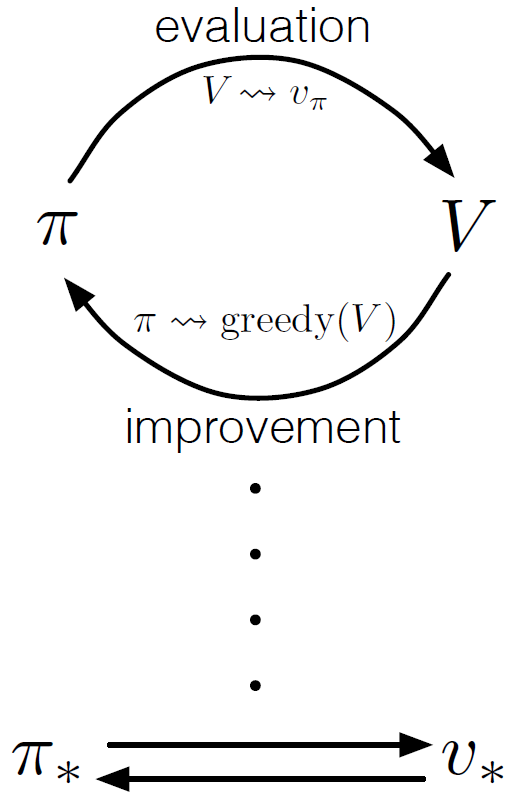
\includegraphics[width=.25\textwidth]{images/gpi}
\caption[Generalised policy iteration]{generalised policy iteration taken from sutton}
\end{wrapfigure}
\end{comment}
\begin{figure}[h]
\centering
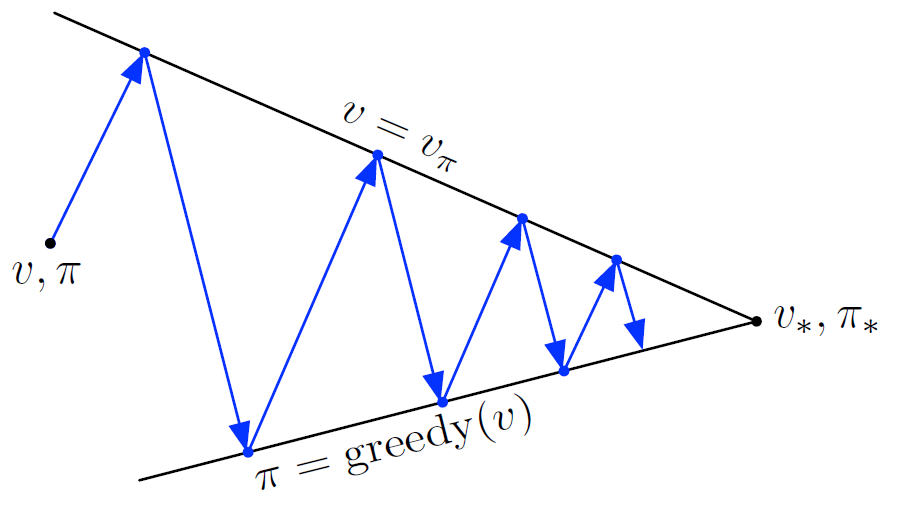
\includegraphics[width=.5\textwidth]{images/gpi2}
\caption[policy and value function convergence]{policy and value function convergence taken from sutton}
\end{figure}
\newpage
\subsection{Monte Carlo}

\begin{wrapfigure}{r}{.27\textwidth}
\vspace{-.6cm}
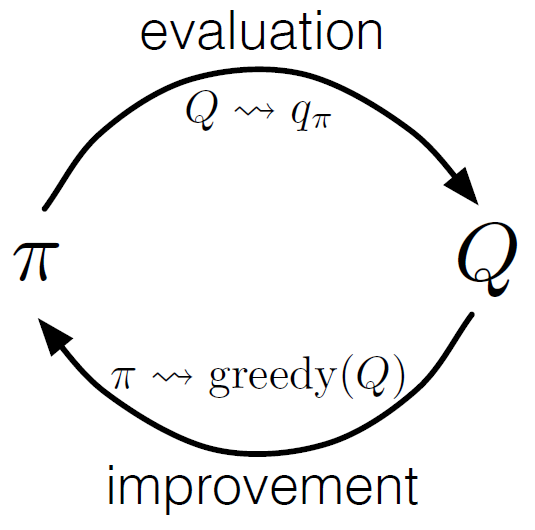
\includegraphics[width=.25\textwidth]{images/gpimc}
\caption[monte carlo policy iteration]{monte carlo policy iteration taken from sutton}
\label{fig:gpimc}
\end{wrapfigure}

\begin{figure}[h]
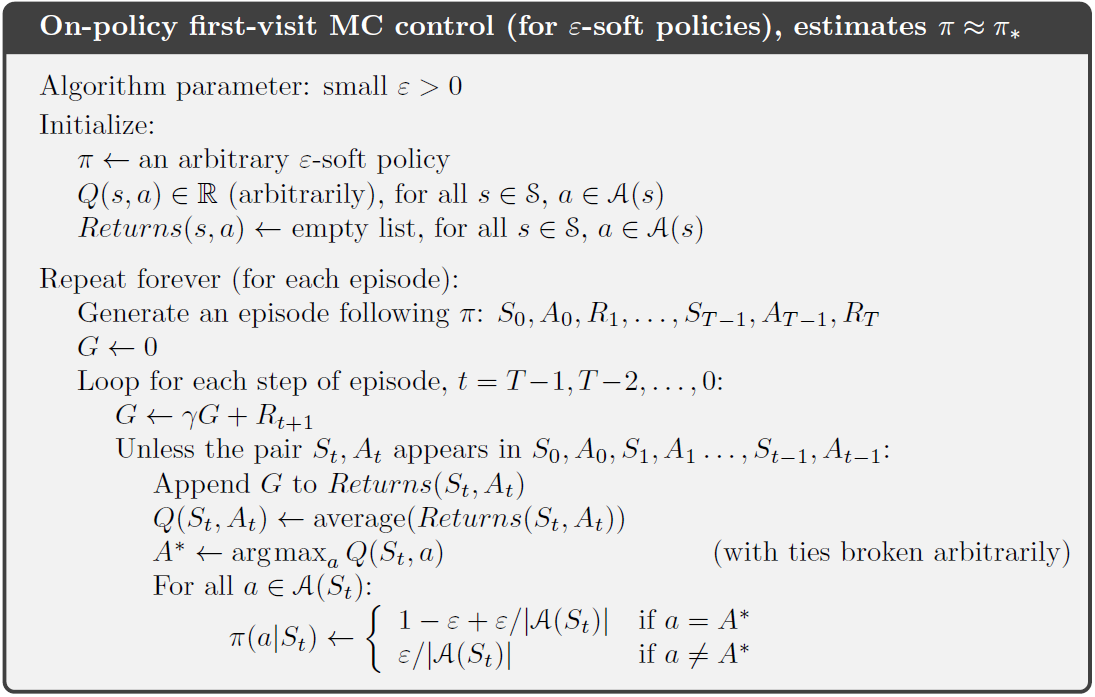
\includegraphics[width=\textwidth]{images/onpolicymc}
\caption[mc algorithm pseudocode]{mc algo pseudocode taken from sutton}
\label{fig:mcsuttonpseudo}
\end{figure}

Monte Carlo methods iterate only at the end of each episode as opposed to every step. This method works by gathering the full return of an episode, and updating the value function of each state that occurred within the episode to reflect this return. Note however it only updates each state once on the first visit, so if a state is visited more than once in an episode, the return is only counted the first time. To ensure all states are explored while maintaining a suitable level of exploitation, Monte Carlo algorithms implement an $\varepsilon$-soft policy, so that the optimal action is taken with a probability of $1-\varepsilon+\varepsilon/|\mathscr{A}\left(S_t\right)|$, where $|\mathscr{A}\left(S_t\right)|$ is the total number of actions, and all other actions are taken with a probability of $|\mathscr{A}\left(S_t\right)|$.
\begin{comment}

"A fourth advantage of Monte Carlo methods, which we discuss later in the book, is
that they may be less harmed by violations of the Markov property. This is because they
do not update their value estimates on the basis of the value estimates of successor states.
In other words, it is because they do not bootstrap." summary ch 5.10 ~\cite{Sutton:RLIntro01}
\end{comment}

\subsection{Q-Learning}

Unlike Monte Carlo, Q-Learning is off-policy, which means the algorithm generally has two policies: one that is used to gather the reward, which is normally a pure greedy function, and another separate policy to gather data, which  explores much more than a typical $\varepsilon$-greedy function. This means the algorithm can effectively explore and exploit simultaneously. Also unlike MC algorithms, Q-learning updates the state-action values after every step, not just at the end of an episode, using the function:

\begin{equation}
Q\left(S_t,A_t\right) \leftarrow \left(1-\alpha\right)Q\left(S_t,A_t\right) + \alpha\left[R_{t+1}+\gamma \max_aQ\left(S_{t+1},a\right)\right]
\end{equation}

\begin{figure}[h]
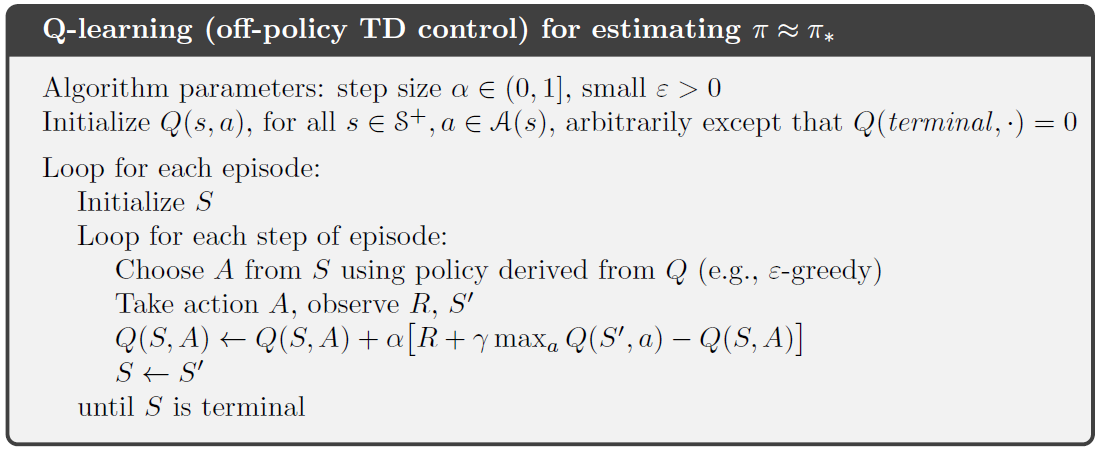
\includegraphics[width=\textwidth]{images/Q-learning}
\caption[Q-learning pseudocode]{Q-learning pseudocode taken from sutton}
\end{figure}

    \chapter{Problem Description}
In order to model a possible workflow, we need to model separate services in an environment. The best way to do this is to build an environment where mathematical operators act as the separate services, and the `ideal workflow' is a function hidden to the learning agent. At the start of each episode, the agent will be given an arbitrary number, and the agent can call one service per timestep in an attempt to reach the correct output value, calculated by the hidden function. The agent will receive a reward of 0 at each timestep until the episode either times out after 20 steps, or reaches the correct value, at which point it will receive a reward inversely proportional to the number of timesteps taken, i.e. $1/n$ where n is the number of operations used. This gives an environment that encourages the agent to to find the correct output in the smallest number of steps, so should learn to avoid circular paths, e.g $+1,-1,+1,-1$. It is important to note that in finding the `ideal' function, the agent may find a function that is different from the hidden function, yet returns the same values; the hidden function could be $x+1\times2$ (ignoring orders of operation, as each step is done separately), yet the agent may find $x\times2+2$, which although `different' does in fact return the same results in the same number of steps. For the purposes of this project, this is unimportant: so long as an `ideal workflow' is found, the specifics of the workflow itself don't matter.

	The most basic environment would include just four basic actions: $+1, -1, \times2$ and $\div2$. Adding additional functions, such as exponents, trigonometric functions, etc. would be trivial, yet add little actual value to the project itself, so only these four basic function types are examined. However, more detailed environments could have a range of discretised values: $+1, +1.1, +1.2...,+5.0$, for each action type, giving a large range of possible actions. This could potentially be expanded further to have multiple continuous action spaces, one for each operator type, with the value being continuous, however, this requires more advanced techniques to solve which are beyond the scope of this dissertation due to time constraint.

The states are very simple within the context of this environment. each state is simply the number of operations that have already been applied within the current episode. This is, however, non-Markov: without knowing the previous operations that have been applied to the input value, there is no way to know if the reward will be reached by performing any given action. Changing the state to include the previous operations will increase the number of states by a factor of at least $O(4^n)$ for each timestep for the most basic environment, more for environments with larger action spaces. Implementing the Markov property for this environment is therefore too computationally expensive to be considered worthwhile. This, combined with the action spaces that are unusually large for typical reinforcement learning problems (most deal with 4 to 5 actions at the most), makes for an environment much more difficult to solve than it may appear from face value. Both non-Markov and large action space environments have yet been fully explored within the Reinforcement learning field, yet are most analogous to real world distributed systems. 


**discussion of application to automated workflow, benefits.

**survey what has been done in field, wolpertinger etc.




    \chapter{Approach}
\begin{comment}
\begin{itemize}
\item mc
\item mc with separate types then speed discarded
\item q learning
\item monte carlo etc
\end{itemize}
non markov - need ones dont use v
\end{comment}

The first part of the approach is to build environments with varying levels of complexity. The first environment, as discussed previously, only requires four basic actions: $+1, -1, \times2$ and $\div2$. The hidden function defining the dynamics of the environment will be a simple two step function, such as $x\times2+1$. This significantly lowers the required number of state-action pairs to be tested before converging to an optimal policy. This can therefore be used to ensure algorithms are implemented properly before moving on to more detailed environments. 

The first algorithm implemented will be a Monte Carlo implementation, as seen in the background materials section. It is important to note that although this is technically a first visit implementation, in this environment no states are visited more than once per episode (recall that the states are the number of operations applied, so will always be $\mathscr{S}=1,2,3,...T$ where $T$ is the terminating state). 

The Monte Carlo implementation was chosen for a multitude of reasons. Firstly, it is a well known, popular algorithm for episodic environments, with a simple theoretical basis to back it mathematically (by law of large numbers, any value will converge eventually to its true value after enough episodes). It is model free, meaning it does not depend on the dynamics of the environment to plan future actions, which is helpful as the non-Markov states for our environment cannot fully predict the future reward. In general, it is one of the algorithms that are least harmed by non-Markov states, in part because it doesn't make use of state value estimates \cite{Sutton:RLIntro115}. Within the `bias-variance tradeoff', Monte Carlo is considered to have no bias (as the values are estimated with actual returns), but a high level of variance, however as the basic environments are made with no noise this isn't a problem.

The other algorithm implemented is Q-learning. Q-learning is an off policy form of temporal difference (TD) learning. Like the Monte Carlo method, Q-learning is a model-free, tabular method. Unlike Monte Carlo methods, TD methods use bootstrapping, which means TD methods update value functions based on the value functions of other states and actions. Also unlike Monte Carlo, Q-learning updates after every step of an episode, as opposed to only at the end of each episode. This can be particularly useful for extended episodes, where waiting for the terminating state would take too much time. Because the environment this project is testing has short episodes, which means updating after every step is unnecessary, and also has non-Markov states, which means bootstrapping will likely backfire, the benefits of Q-learning will be negligible and the disadvantages will be pronounced. Nonetheless, it is helpful to implement this algorithm to display how choice of algorithm can drastically effect the outcome, depending on the properties of the environment.

Once these are implemented for the most basic environment, they will again be implemented for the environments with further complexity. in these environments, the values of each possible operation range from 1.0 to 5.0, discretised at varying values. This increases number of states significantly, and so will increase the learning time. Additionally, more complex functions will be tested, with multiple steps required, again to test the learning time.
    \chapter{Application of Approach}

A proportion of the project time was spent researching reinforcement learning, in order to obtain the grounding required to design the environments, choose appropriate algorithms and implement them. Approximately three weeks were spent reading Sutton and Barto's `Introduction to Reinforcement Learning'\cite{Sutton:RLIntro01} cover to cover, and watching the DeepMind lecture series \cite{silver}. 

Next was designing the environment itself. An open source python library called OpenAI Gym was used to create the environments \cite{AIgym}. OpenAI Gym is a package that provides multiple pre-made environments to test reinforcement learning methods, but also allows for the creation of custom environments. By using gym we can ensure the environment's design is standardized to work in RL field, as well as use base functions within Gym, to make implementation faster. Nearly two weeks were spent learning the code base and learning how to use Gym, and two weeks were spent designing and implementing the different environments.

\begin{figure}[h]
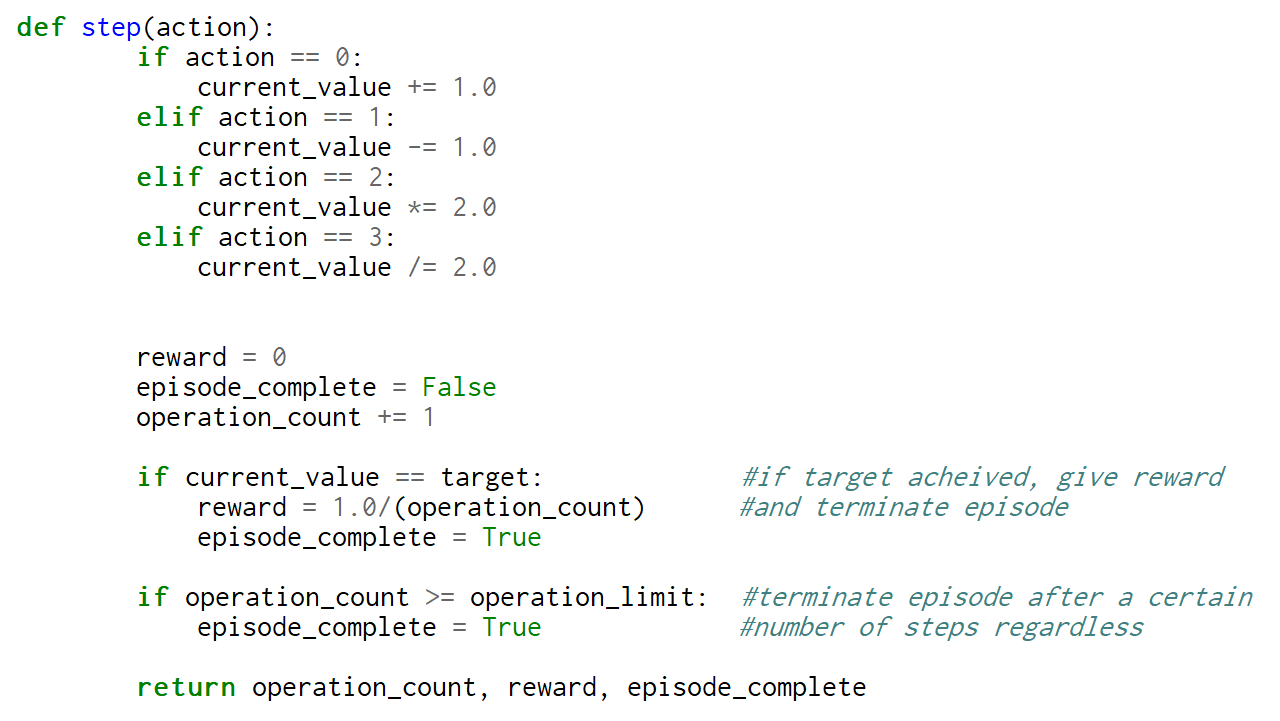
\includegraphics[width=\textwidth]{images/pseudo}
\caption[basic environment pseudocode]{pseudocode for the step function within the basic environment}
\label{fig:basicenv}
\end{figure}

Figure \ref{fig:basicenv} shows pseudocode of the step function for the most basic environment. Note that the possible actions are provided in the form of integers, 0 to 4. If the target is achieved or the limit of operations is hit the episode terminates. The reward is 0 if the target is not achieved, or a value of $1/n$, where $n$ is the number of operations taken to reach the target. The return is operation\_count (which is the state of the environment), the reward, and a boolean that determines whether or not the episode has terminated. 

\begin{figure}[h]
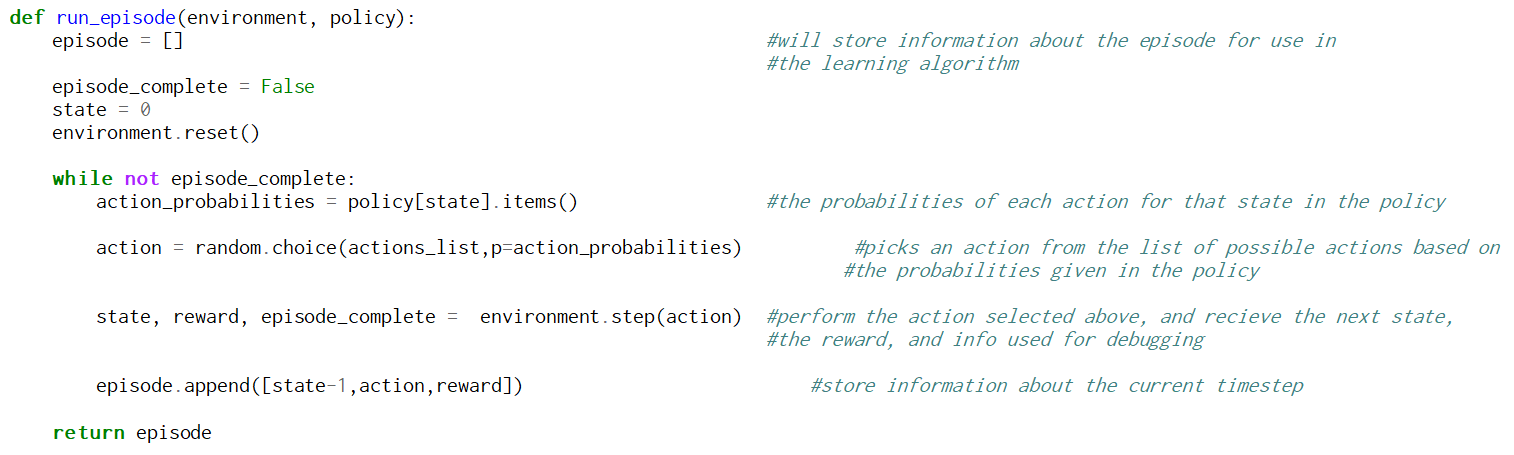
\includegraphics[width=\textwidth]{images/run}
\caption[run episode pseudocode for Monte Carlo]{pseudocode for running a single episode of an environment for the Monte Carlo algorithm}
\label{fig:mcrun}
\end{figure}

\begin{figure}[h]
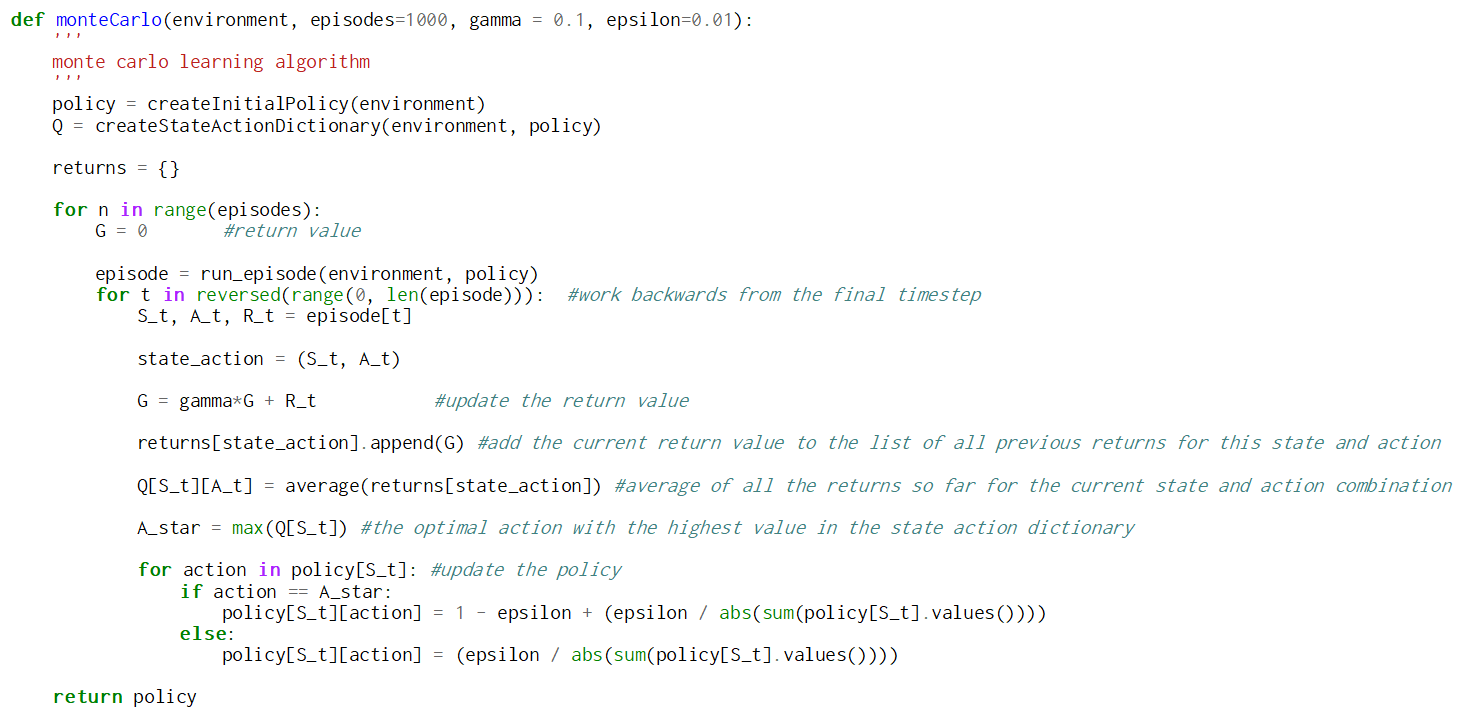
\includegraphics[width=\textwidth]{images/mcpseudo}
\caption[Monte Carlo implementation pseudocode]{pseudocode of the Monte Carlo first visit algorithm}
\label{fig:mcpseudo}
\end{figure}
Figure \ref{fig:mcrun} shows pseudocode of a basic function that runs an episode of an environment given a policy. The action is chosen based on the probabilities given within the provided policy. The state, action, and resulting reward are then stored for each timestep to be used within the Monte Carlo algorithm. Figure \ref{fig:mcpseudo} shows the pseudocode for the implementation. Note that unlike in figure \ref{fig:mcsuttonpseudo} this implementation does not have a check to see if the state has been previously visited in the episode before updating the returns list and the policy. This is due to the type of states within this environment - as each state is simply the number of operations performed, it is therefore clear that no state can be visited twice per episode, as the state will always increment with each timestep. This check can therefore be removed without affecting the underlying process.

For Q-learning, the behaviour policy (the policy used to generate data to update the reward policy) was an epsilon greedy policy, and the reward policy was a pure greedy policy. Instead of updating at the end of each episode, this policy updates after each step, as seen in figure \ref{fig:Qpseudo}.
\begin{figure}[h]
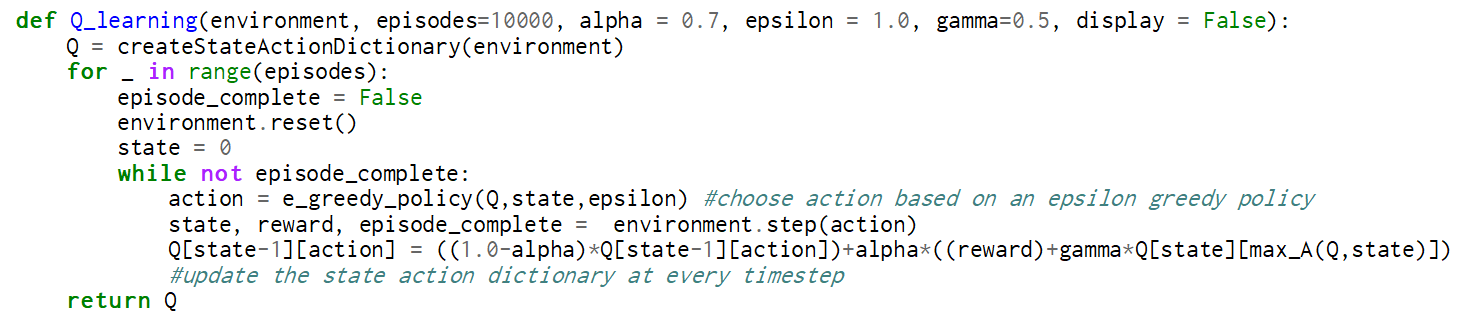
\includegraphics[width=\textwidth]{images/Qpseudo}
\caption[Q-learning implementation pseudocode]{pseudocode of the Q-learning implementation}
\label{fig:Qpseudo}
\end{figure}


    \chapter{Results}
Monte Carlo for the basic environment with 4 possible actions is shown in figure \ref{fig:mcbasicfull}. The rewards were normalised so the ideal workflow every time gives a reward of 1.0. For this algorithm $\gamma=1.0$ and $\varepsilon=0.01$. It is clear from the figure that Monte Carlo works optimally: it learns quickly (levelling off within 500 episodes) and returns a high average reward. This is expected as Monte Carlo is designed to work well with episodic environments, and has a low bias.
\begin{figure}[h]
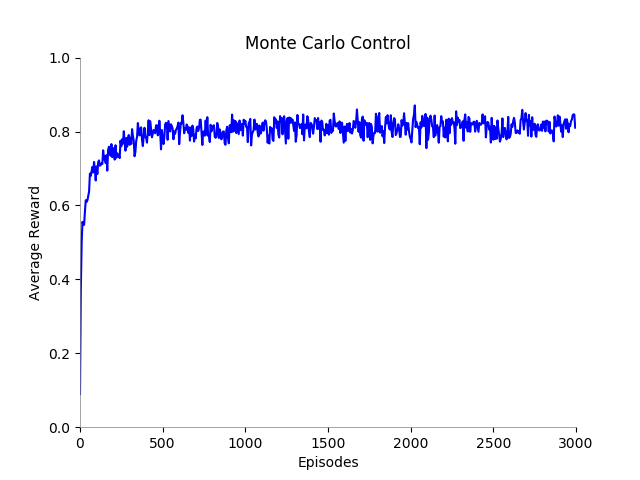
\includegraphics[width=\textwidth]{resultsbasic/21_100runs_3000_normalised}
\caption[Monte Carlo Control for Basic Environment]{Monte Carlo control averaged over 100 runs for an environment with 4 possible actions, normalised to true reward on optimal behaviour}
\label{fig:mcbasicfull}
\end{figure}

Q-learning, on the other hand, is not well suited to this environment with non-Markov states. As can be seen in figure \ref{fig:qgraph}, the algorithm levels off at a reward level of only 20\% of the true reward value. Because of such poor results for the basic environment, Monte Carlo was the main focus for the remainder of the trials.
\begin{figure}[h]
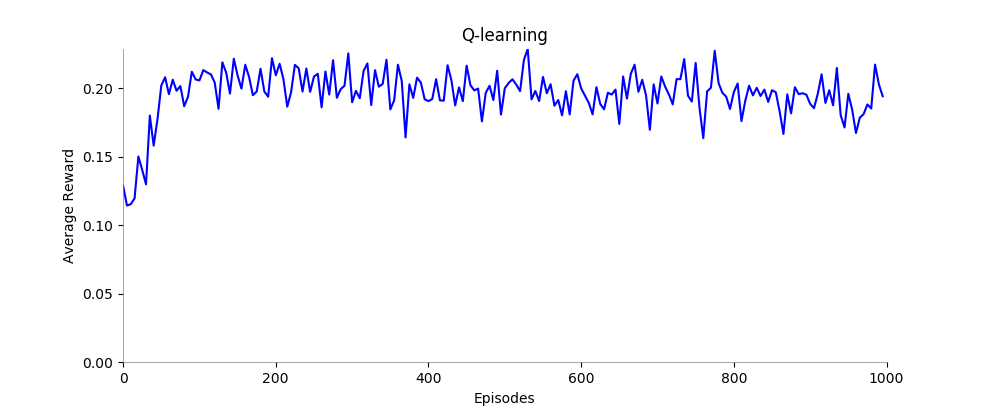
\includegraphics[width=\textwidth]{resultsq/basic10002}
\caption[Q-learning for the basic environment]{Q-learning averaged over 1000 runs for an environment with 4 possible actions, normalised to true reward}
\label{fig:qgraph}
\end{figure}

\begin{comment}
\begin{figure}[h]
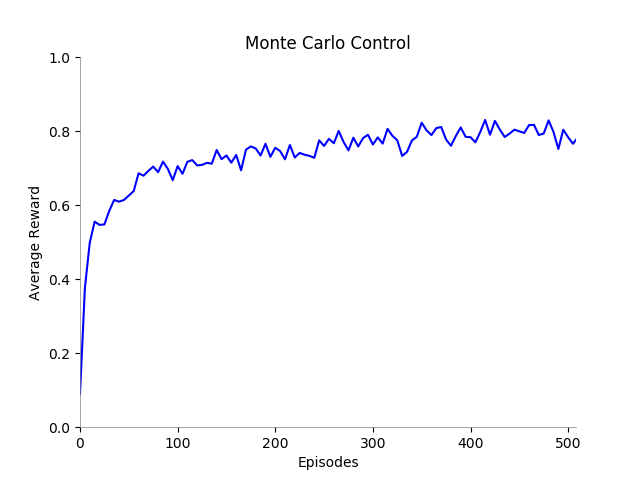
\includegraphics[width=\textwidth]{resultsbasic/21_100runs_500normalised}
\caption[Monte Carlo Control for Basic Environment]{Monte Carlo control averaged over 100 runs for an environment with 4 possible actions, normalised to true reward on optimal behaviour}
\label{fig:mcbasiczoom}
\end{figure}
\end{comment}

Figure \ref{fig:diffgammas} shows the effects of a different $\gamma$ choice. Recall from section \ref{MDP} that $\gamma\in\left(0,1\right]$ is the discount factor, and a smaller discount factor emphasises immediate reward.
\begin{figure}[h]
\centering
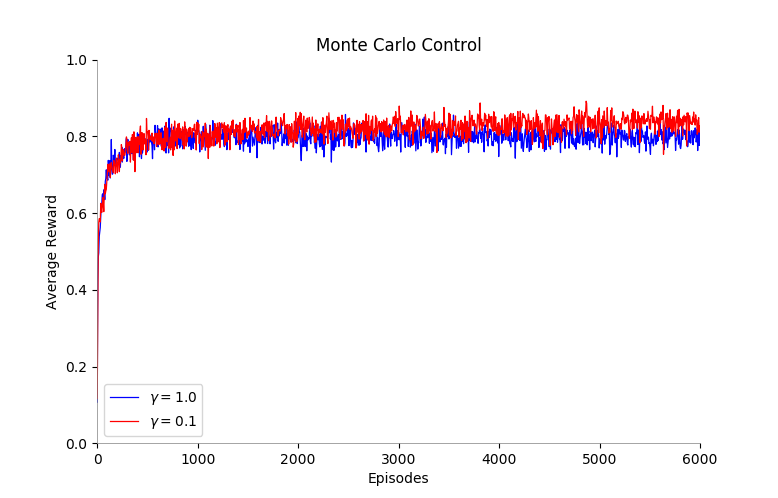
\includegraphics[width=.85\textwidth]{resultsbasic/differentgammas}
\caption[Monte Carlo Control]{Monte Carlo control averaged over 100 runs for an environment with 4 possible actions, with different choices of $\gamma$}
\label{fig:diffgammas}
\end{figure}

As the environment only provides a reward once at the end of an episode, and we are looking to find paths with the least amount of time steps, it is logical to choose a smaller discount factor (to emphasize the preference for immediate reward). Although a smaller discount factor means the algorithm learns (marginally) slower, it also means the eventual average reward is higher, and is therefore the optimal choice for an environment of this style.
\begin{figure}[h]
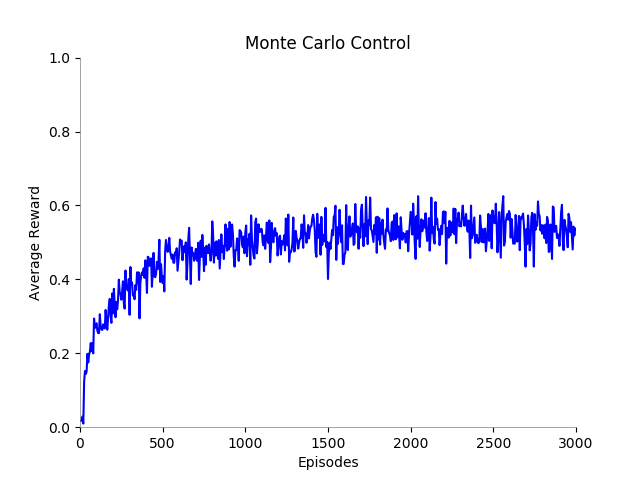
\includegraphics[width=\textwidth]{resultsdiscretemc/41100runs3000normalised}
\caption[Monte Carlo Control for Discretised Environment]{Monte Carlo control averaged over 100 runs for an environment with 20 possible actions}
\label{fig:discrete}
\end{figure}

With the action space expanded for the discretised environment, the average reward lowers as expected. In figure \ref{fig:discrete} is the Monte Carlo control for an environment that has 20 possible actions: the four original operators, with the possible values $1.0,2.0,3.0,4.0$ and $5.0$. The hidden function is still a basic two step function (this time $-1.0\times4.0$). The algorithm still achieves a good learning rate, although not as fast as the previous  
\begin{comment}
\begin{figure}[h]
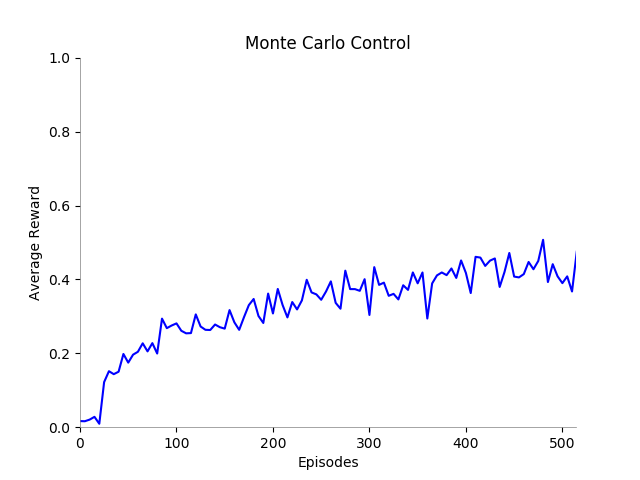
\includegraphics[width=\textwidth]{resultsdiscretemc/41_100runs500normalised}
\caption[Monte Carlo Control for Discretised Environment]{Monte Carlo control averaged over 100 runs for an environment with 20 possible actions}
\end{figure}
\end{comment}
\begin{figure}[h]
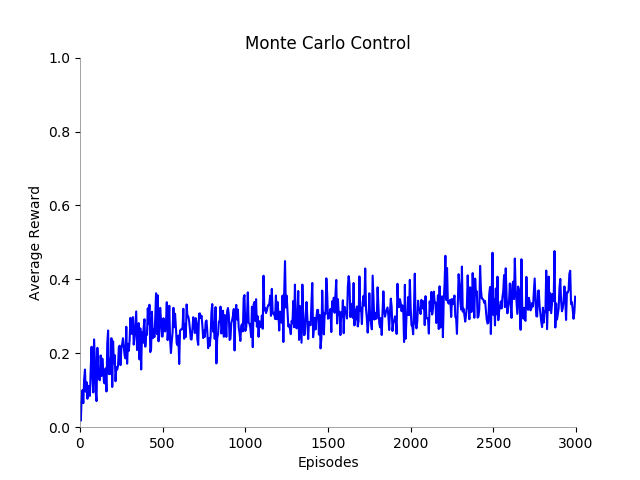
\includegraphics[width=\textwidth]{resultscomplexmc/413_100runs_3000normalised}
\caption[Monte Carlo Control for the discretised environment with complex function]{Monte Carlo control averaged over 100 runs for an environment with 20 possible actions, learning a more complex hidden function}
\end{figure}

\begin{figure}[h]
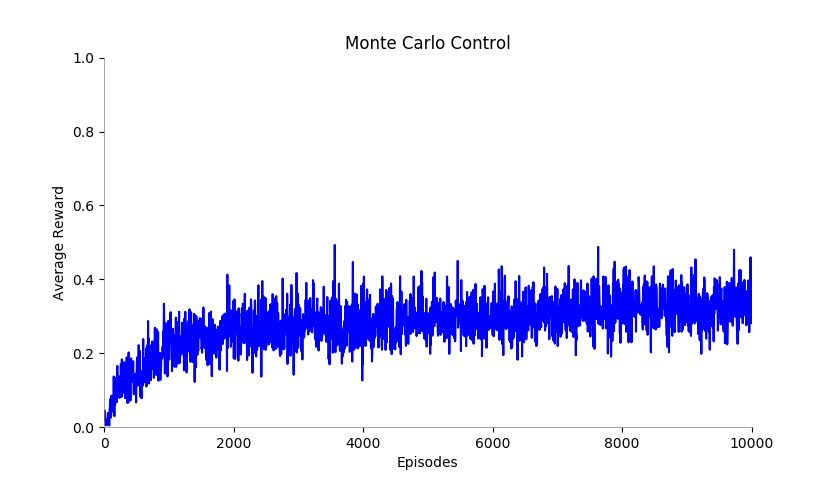
\includegraphics[width=\textwidth]{discretequarter/figure_1}
\caption[Monte Carlo Control for the discretised environment with 68 actions]{Monte Carlo control averaged over 100 runs for an environment with 68 possible actions}
\end{figure}








    \chapter{Analysis}

    \chapter{Conclusions}

    \chapter{Reflection}

    
	\SgIncludeBib{biblio}
\end{document}